% Document Class and packages
\documentclass[a4paper, 12pt]{memoir}
\usepackage{subfiles}
\usepackage[utf8]{inputenc}
\usepackage[italian]{babel}
\usepackage{microtype}
\usepackage{graphicx}
\usepackage[usenames,dvipsnames,svgnames,table]{xcolor}
\usepackage[a4paper, bindingoffset=1cm]{geometry}
\usepackage{cite}
\usepackage{hyperref}
\usepackage{float}
\usepackage{caption}

% Increase space between paragraphs
\setlength{\parskip}{3pt}
% increase space between lines
\linespread{1.2}

% about:author
\author{Paolo Scaramuzza}
\title{Studio dell' efficienza di oscillatori LC integrati per impulsatori 
	Ultra Wideband}
\date{} % HACK: avoids date in the title

\begin{document}
\subfile{tex/front} % make a nice front page (thanks HammondSmoking)

%%%%%%%%%%%%%%%%%%%%%%%%%%%%%
% Abstract
%%%%%%%%%%%%%%%%%%%%%%%%%%%%%
\cleardoublepage{}
\newpage
\pagenumbering{gobble} % no need for numbering
\begin{vplace}[0.7]
	\subfile{tex/abstract}
\end{vplace}
%%%%%%%%%%%%%%%%%%%%%%%%%%%%%
% Index
%%%%%%%%%%%%%%%%%%%%%%%%%%%%%
\cleardoublepage{}
\newpage
\tableofcontents

\pagenumbering{arabic} % restore normal page numbering
%%%%%%%%%%%%%%%%%%%%%%%%%%%%%
% Introduzione
%%%%%%%%%%%%%%%%%%%%%%%%%%%%%
\chapter{Introduzione}
Contrariamente a molte tecnologie in radiofrequenza oggi in uso, la radio a
impulsi Ultra-Wideband (\emph{Ultra-Wideband Impulse-Radio}, UWB IR)
sfrutta un' ampia porzione dello spettro delle radiofrequenze (di ampiezza
maggiore a 500MHz oppure più del 25\% della frequenza di centro-banda
\cite{Neviani12}) trasmettendo i dati sotto forma di impulsi di breve durata.\\
Tra gli schemi di modulazione impiegati si trovano: 
\begin{itemize}
	\item \emph{on-off keyng} (OOK)
	\item \emph{pulse-position modulation} (PPM)
\end{itemize}

Per molti anni la UWB IR è stata impiegata esclusivamente in ambito
militare. Nel 2002, con la regolamentazione dello spettro di frequenze tra 3.1 
e 10.6GHz da parte degli Stati Uniti e in seguito dall'Europa e dal Giappone,
la radio UWB ha iniziato ad affermarsi quale soluzione più conveniente, sia dal
punto di vista economico che prestazionale, per la comunicazione a corto raggio.
\\La massima densità spettrale di potenza in trasmissione consentita dalle
leggi europee è di $ -41.3 dBm/MHz $ e in alcuni segmenti dello spettro tale
limite può arrivare fino a $ -75 dBm/MHz $, come evidenziato in\cite{Hirt07}.\\
Vista la bassa potenza di trasmissione e le elevate frequenze operative,
le radio a impulsi UWB ben si prestano ad essere realizzate interamente in
tecnologia CMOS.\@
Si possono avere così trasmettitore e ricevitore in un unico circuito integrato.
\\Tra le possibili applicazioni di questa tecnologia si trovano: la
localizzazione di precisione e la trasmissione a corto raggio.

Per la localizzazione si cita\cite{Terada05} in cui si mostra una radio 
Ultra-Wideband realizzata in tecnologia CMOS da $ 180nm $ in grado di
effettuare localizzazioni a più di un metro di distanza con un errore massimo
di $ \pm 2.5cm $.
Quando si effettuano mille misurazioni al secondo il consumo di potenza è pari
a $ 0.7\mu W $. Il trasmettitore e il ricevitore sono integrati in un unico
chip avente un' area di $ 0.415mm^2 $.

Per la trasmissione a corto raggio significativi risultati sono stati raggiunti
da\cite{RabaeyEECS},\cite{Neviani12} e\cite{Gambini12} in cui sono dimostrate
varie soluzioni circuitali che permettono di ottenere, in un unico circuito
integrato di piccole dimensioni, sia la funzionalità di trasmettitore che di
ricevitore.

Attualmente la frontiera della ricerca si sta spostando verso una sempre
maggiore integrazione e un miglioramento globale dell'efficienza energetica.
Questi risultati della Ricerca permettono di avere radio dalla durata della 
batteria estremamente lunga o di far funzionare la circuiteria tramite
\emph{energy harvesting}.\\
Un esempio significativo è\cite{Danesh11} in cui si ha un nodo sensore 
alimentato da un pannello solare di $ 2\times2 cm^2 $ che svolge anche la
funzione di antenna. Il sensore è poco più grande del pannello solare, consuma
solamente $ 10\mu W $ di potenza e trasmette i dati a intervalli di un
minuto alla velocità di $ 1 KB/s $ tramite la modulazione \emph{on-off
keying}.
Con l'impiego di un supercondensatore, inoltre, è in grado di lavorare in
condizioni di totale assenza di illuminazione per più di due giorni.\\
In\cite{Solda10} infine è dimostrata la realizzazione di una radio a impulsi 
che garantisce un' efficienza in trasmissione pari al 7\% mentre in 
\cite{Neviani14} si raggiunge l'~$11,7\%$, valore che rappresenta l'attuale
stato dell'arte.

La presente tesi parte proprio dai risultati ottenuti in~\cite{Neviani12} e
\cite{Neviani14} e mira a massimizzare l'efficienza energetica dell'oscillatore
LC \emph{cross-coupled} in uso nell'impulsatore.

In Figura 1.1 è rappresentato lo schema elettrico di un oscillatore LC
\emph{cross coupled} nella sua forma più semplice.\\
\begin{figure}[h]
\centering
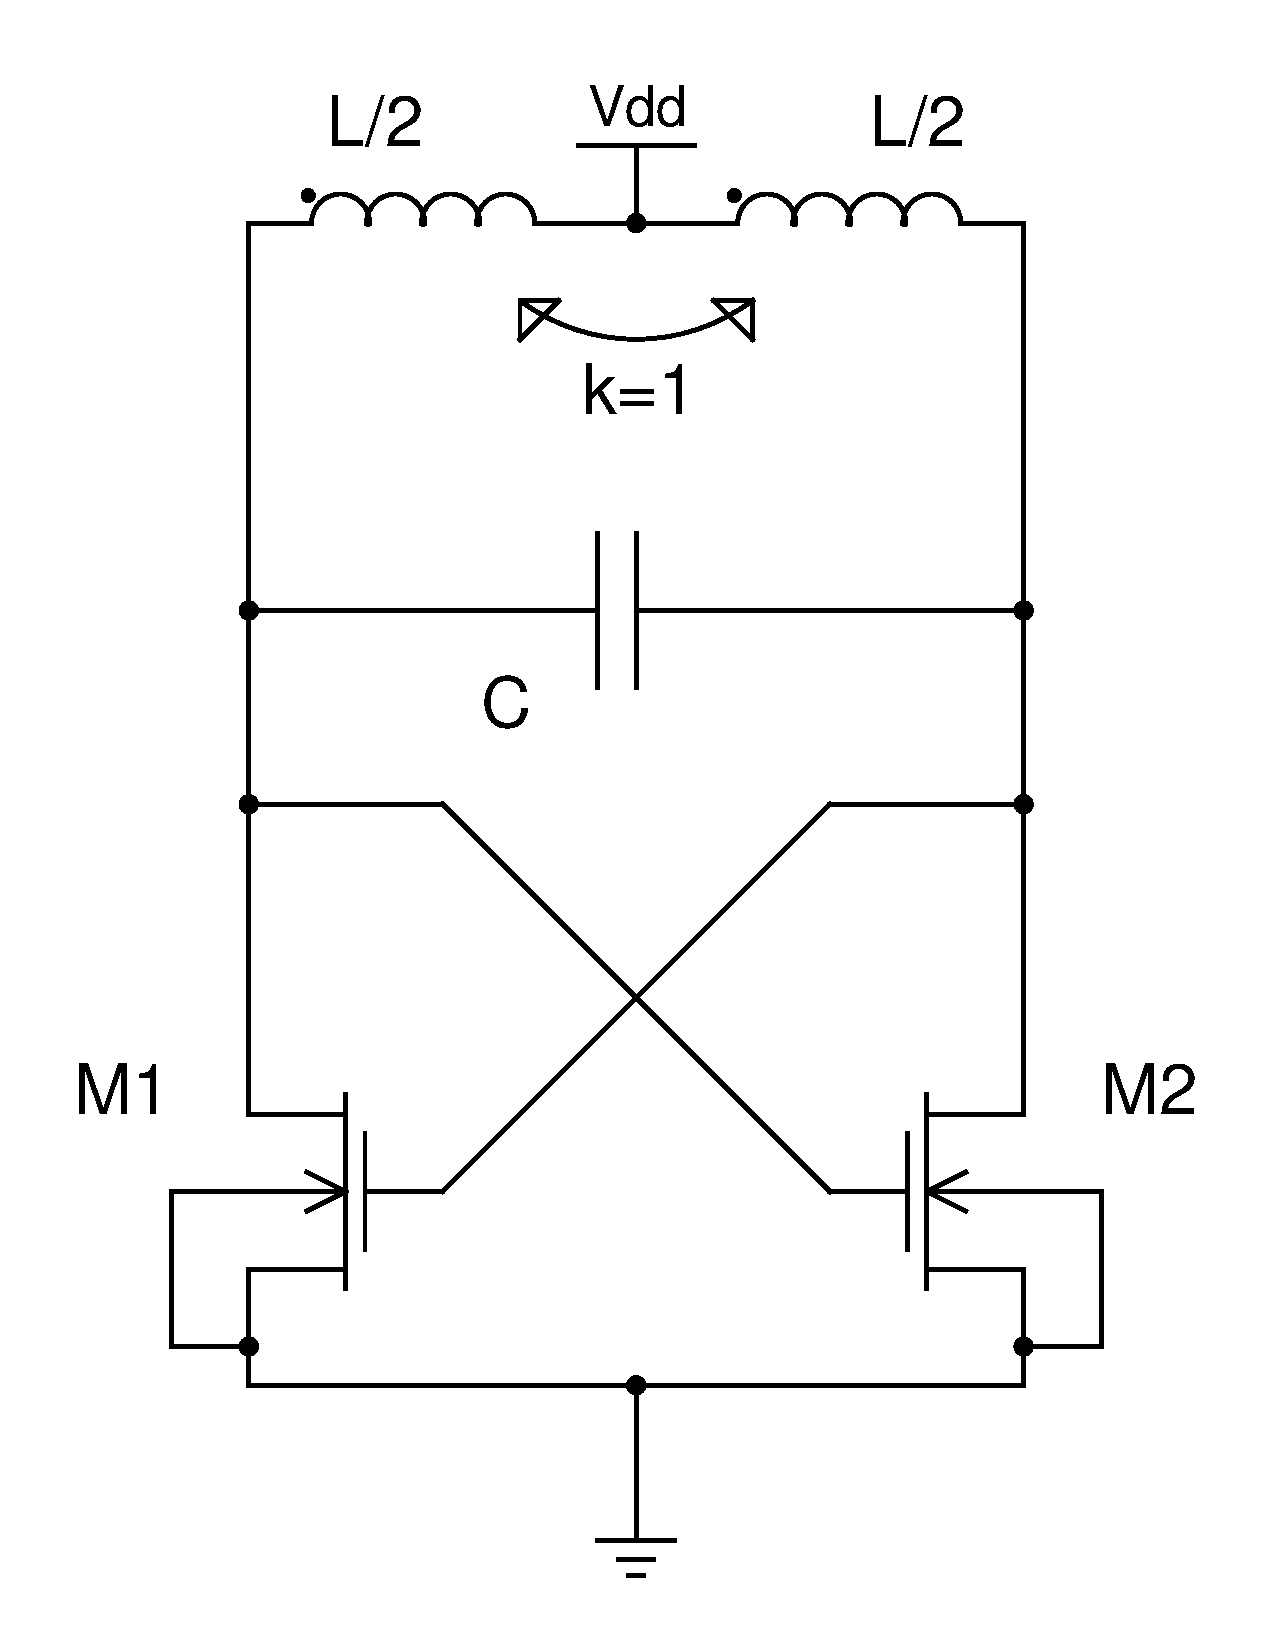
\includegraphics[width=0.34\textwidth]{images/LCosc.pdf}
\caption{Schema elettrico dell'oscillatore LC \emph{cross-coupled}}
\end{figure}
\`E la tipologia di oscillatore più diffusa nei circuiti integrati perché il
rumore di fase è più basso rispetto ad altre soluzioni e richiede un basso
numero di componenti attivi\cite{Amran05}\cite{RazaviRF}.

Il suo funzionamento si basa sulla risonanza tra l'induttanza e la capacità
presenti nel circuito. \\
Gli NMOS del circuito infatti formano una coppia incrociata e ognuno dei due
rami apporta, come si evince dai diagrammi di Bode in Figura 1.2, uno
sfasamento di $ 180^{\circ} $ alla pulsazione $ \omega _r=\frac{1}{\sqrt{LC}} $.

Per il singolo ramo del circuito, detta $ R_p $ la resistenza parassita
complessiva e $ g_m $ la transconduttanza del MOSFET, si ha la seguente
funzione di trasferimento:
\begin{center}
$ W(s)=\frac{V_{out}}{V_{in}}=-g_m Z(s)=-g_m \frac{R_p L s}{R_p C L s^2 + Ls + R_p} $
\end{center}

\begin{figure}[h]
\centering
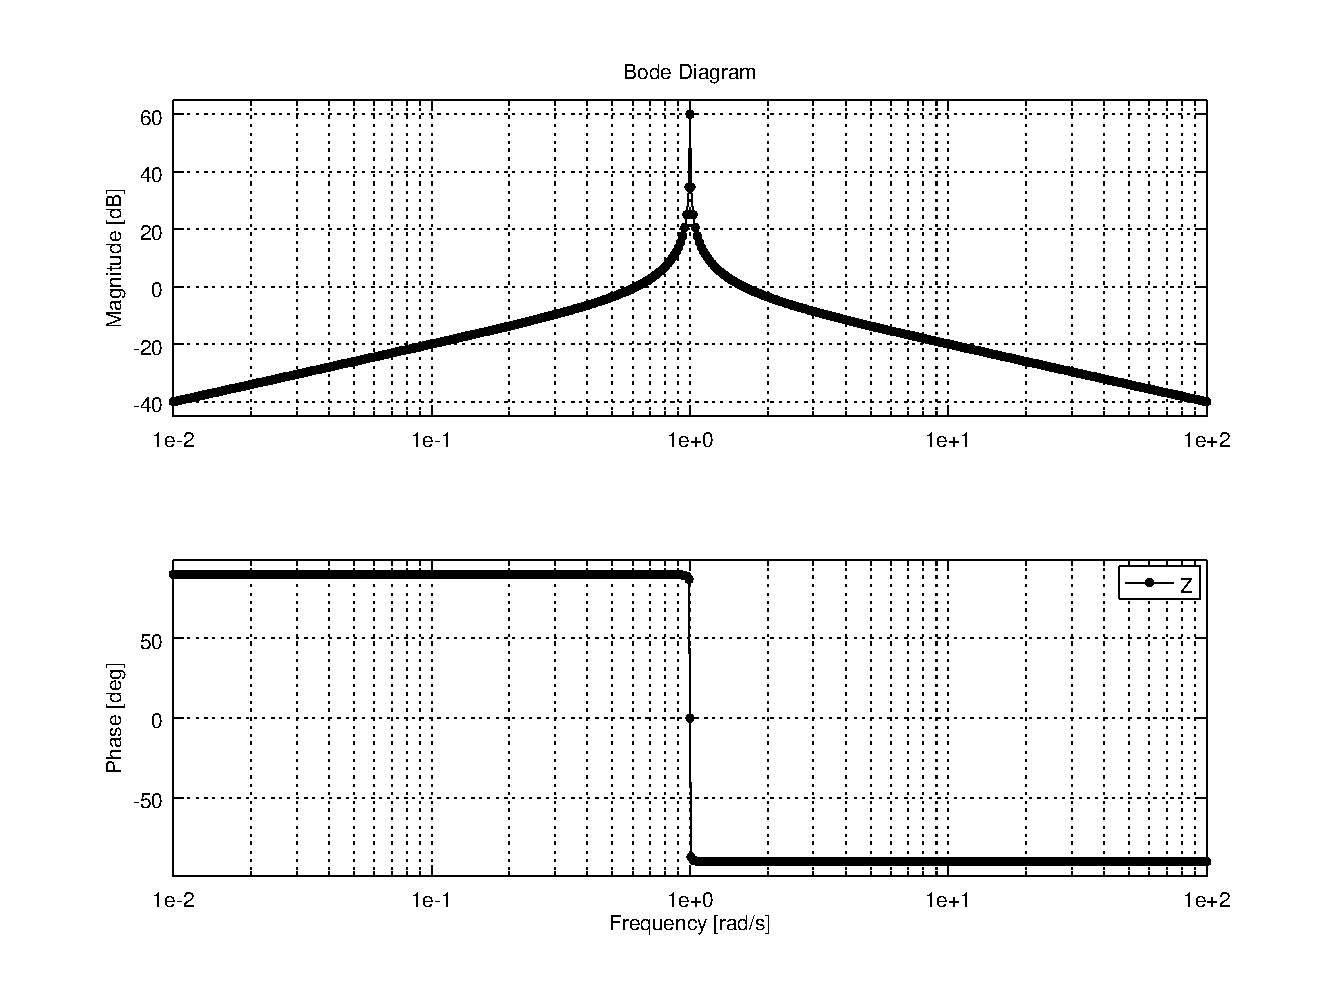
\includegraphics[width=\textwidth]{images/BodeLC.pdf}
\caption{Diagramma di Bode per $ Z(s) $ con $L=1H$, $C=1F$ e $R_p=1K\Omega$}
\end{figure}

In considerazione della $ W(s) $ sopra descritta è possibile applicare il
criterio di Barkhausen\cite{JaegerMicro} che afferma che il circuito si
comporta da oscillatore se alla pulsazione $ \omega _r $ il modulo della
funzione di trasferimento in catena aperta è pari ad uno e lo sfasamento è di
$ 360^{\circ} $.\\
Per avere oscillazione è dunque necessario porre in cascata, chiudendo l'
anello di retroazione, due stadi del tipo di circuito presentato in Figura 1.3,
assicurandosi che $ {\left( g_m R_p \right)}^2 = 1 $ 
\cite[p.652]{RazaviFundamentals}.\\
Riorganizzando lo schema circuitale si riottiene quello in Figura 1.1.

\begin{figure}[h]
\centering
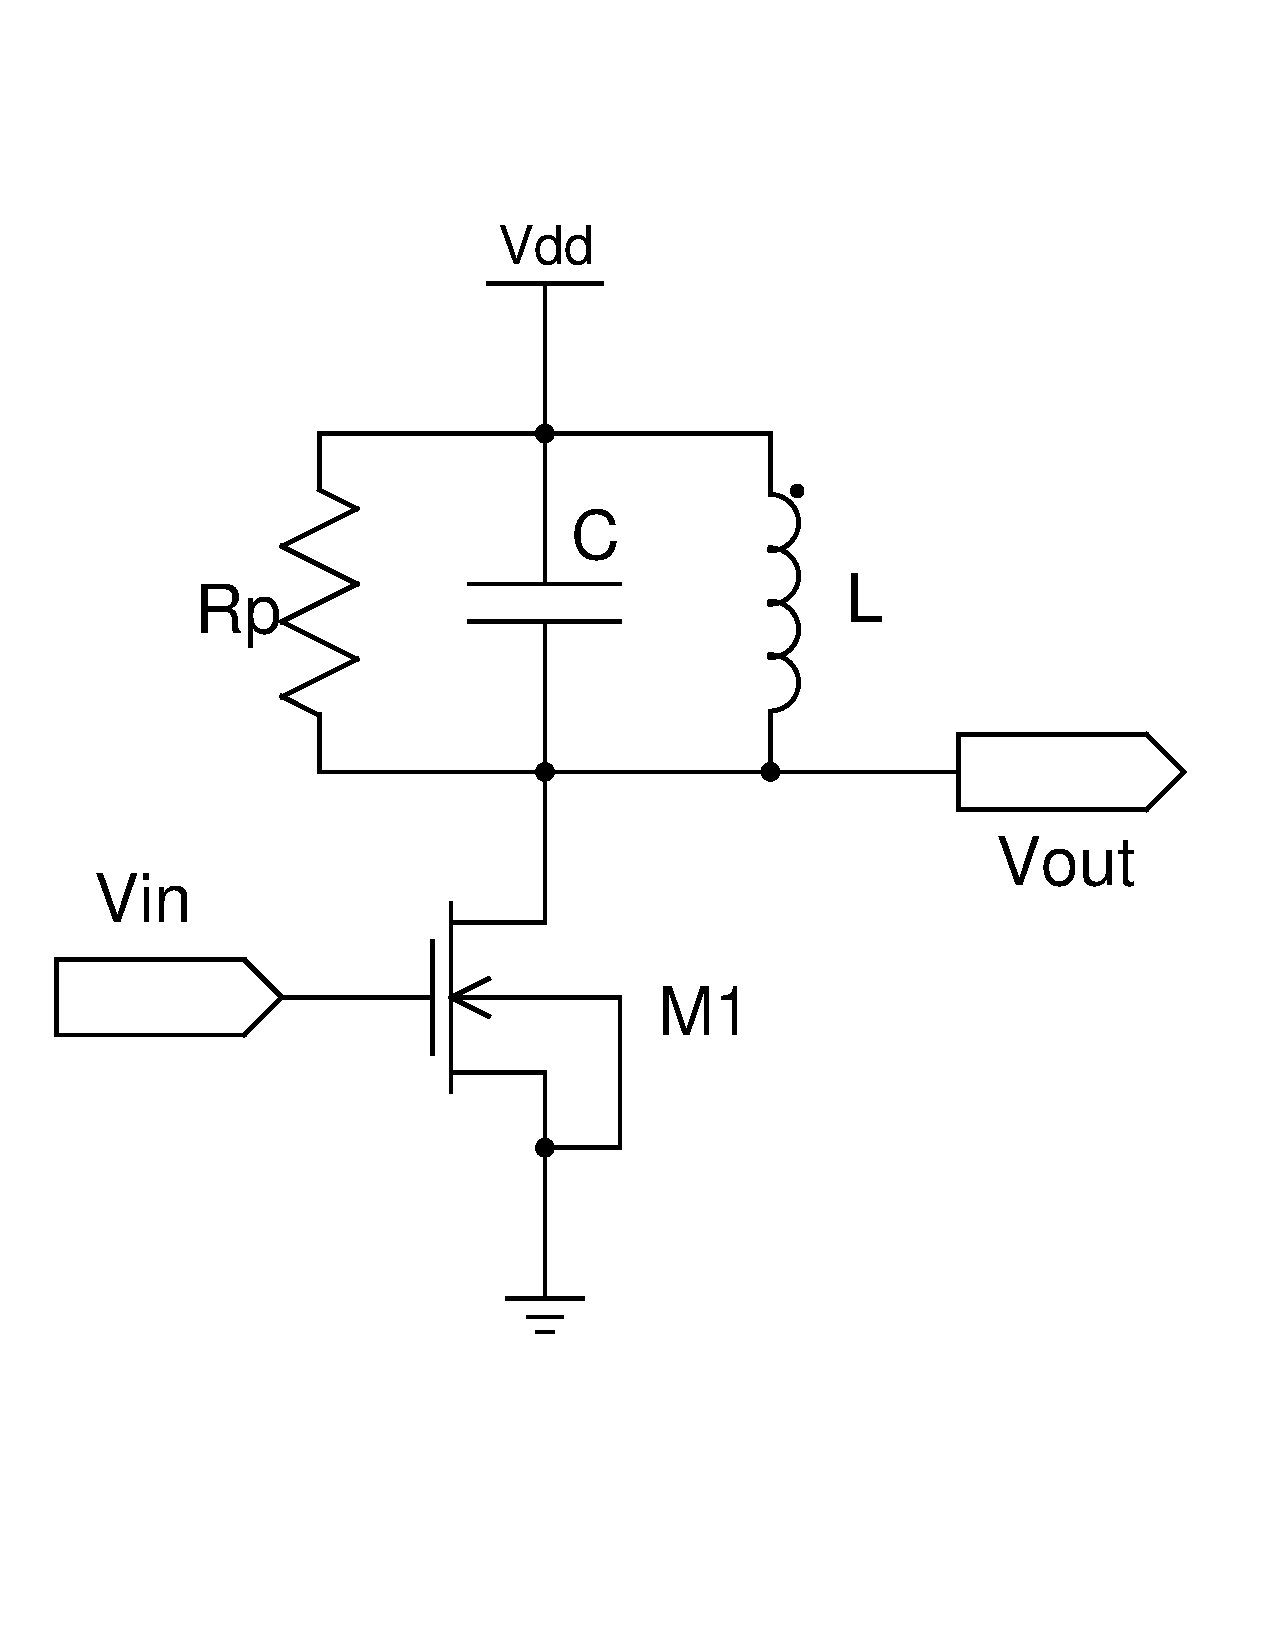
\includegraphics[width=0.5\textwidth]{images/LCsingle.pdf}
\caption{Schema per il singolo ramo dell'oscillatore}
\end{figure}

\section{Contributi della tesi}
Nell'ambito del lavoro svolto i valori dell'induttanza e della capacità sono
tarati in modo tale da produrre un' onda sinusoidale alla frequenza di 8GHz.\\
L'induttanza è sostituita da un trasformatore al cui secondario è collegata
l'antenna. La circuiteria di controllo aggiunta si occupa di attivare e
disattivare l'oscillatore per produrre gli impulsi.

Un modello teorico semplificato per il circuito è stato ricavato approssimando
i MOSFET come dei generatori ideali di tensione alternata ad 8GHz
connessi al primario del trasformatore. \\
Tale modello ha permesso di valutare in prima approssimazione l'effetto sul
comportamento del circuito delle variazioni nel dimensionamento dei componenti.

Partendo dai valori ottenuti in\cite{Neviani14} si è poi effettuata la
simulazione al calcolatore del circuito a livello di transistor.\\
Si è evidenziato che, a meno di effetti di ordini successivi al primo, i
risultati della simulazione sono in accordo con il modello teorico.\\
Affinando le indicazioni del modello tramite il calcolatore, si sono
raggiunti valori di efficienza massima per il circuito simulato nell'intorno
del 29\%, partendo da un valore iniziale pari al 10\%.\\
Le simulazioni effettuate su trasformatore da solo confermano ulteriormente i
risultati ottenuti.

Si presentano e discutono infine i massimi valori di efficienza raggiunti nelle
simulazioni dalle due topologie ed è illustrato come queste differiscano poco 
l'una dall'altra dal punto di vista dell'efficienza. \\
La scelta di un tipo di oscillatore piuttosto che l'altro deve dunque essere
dettata da altri parametri (ad esempio l'occupazione di area ed il consumo
dinamico di potenza) che esulano dal contributo di questa tesi e sono solo
accennati.
\newpage
\section{Struttura dell'elaborato}
Il presente elaborato è organizzato come segue:
\begin{itemize}
\item nel Capitolo 2 sono presentate le due diverse tipologie di oscillatore
	prese in esame. \`E discusso come da essi si giunga ad un modello
	semplificato e si presenta un'analisi qualitativa degli effetti
	sull'efficienza del diverso dimensionamento dei componenti nel
	modello ottenuto.
\item Nel Capitolo 3 sono presentati e discussi i risultati numerici delle
	simulazioni, confrontando le diverse topologie dell'oscillatore.
\item Il Capitolo 4 è dedicato agli sviluppi futuri e alla discussione dei
	parametri di interesse la cui valutazione si presta ad ulteriori studi.
\end{itemize}
%%%%%%%%%%%%%%%%%%%%%%%%%%%%%
% Tipologie e parametri
%%%%%%%%%%%%%%%%%%%%%%%%%%%%%
\chapter{Topologie e parametri di interesse}
Come è stato descritto nel capitolo precedente, sono stati analizzati due
diversi oscillatori LC in topologia \emph{cross coupled} per la realizzazione di
impulsatori ultra-wideband.

\section{Le topologie}
In Figura 2.1 è presentato lo schema dell'oscillatore denominato di Tipo 1.\\
Alla topologia basilare è aggiunto un NMOS (indicato con M3) con
drain e source connessi tra l'oscillatore e la massa. L'accensione e lo
spegnimento avvengono fornendo al gate di M3 un valore logico rispettivamente
alto e basso.\\
Quando M3 è spento, ovvero quando la tensione tra gate e drain è
nulla, esso si comporta come un circuito aperto e dunque l'oscillatore non
viene alimentato. Quando invece M3 è in saturazione, ovvero quando la tensione 
al gate supera la tensione di soglia, la sua resistenza è molto bassa, dunque 
il circuito viene chiuso e l'oscillatore inizia a funzionare.

In Figura 2.2 è presentato lo schema dell'oscillatore denominato di Tipo 2.\\
Rispetto alla soluzione precedente una coppia di invertitori in logica
complementare è connessa ai gate degli NMOS dell'oscillatore. L'accensione e
lo spegnimento avvengono quando all'ingresso degli invertitori si presenta un
valore logico rispettivamente basso o alto.

\begin{figure}[h]
\centering
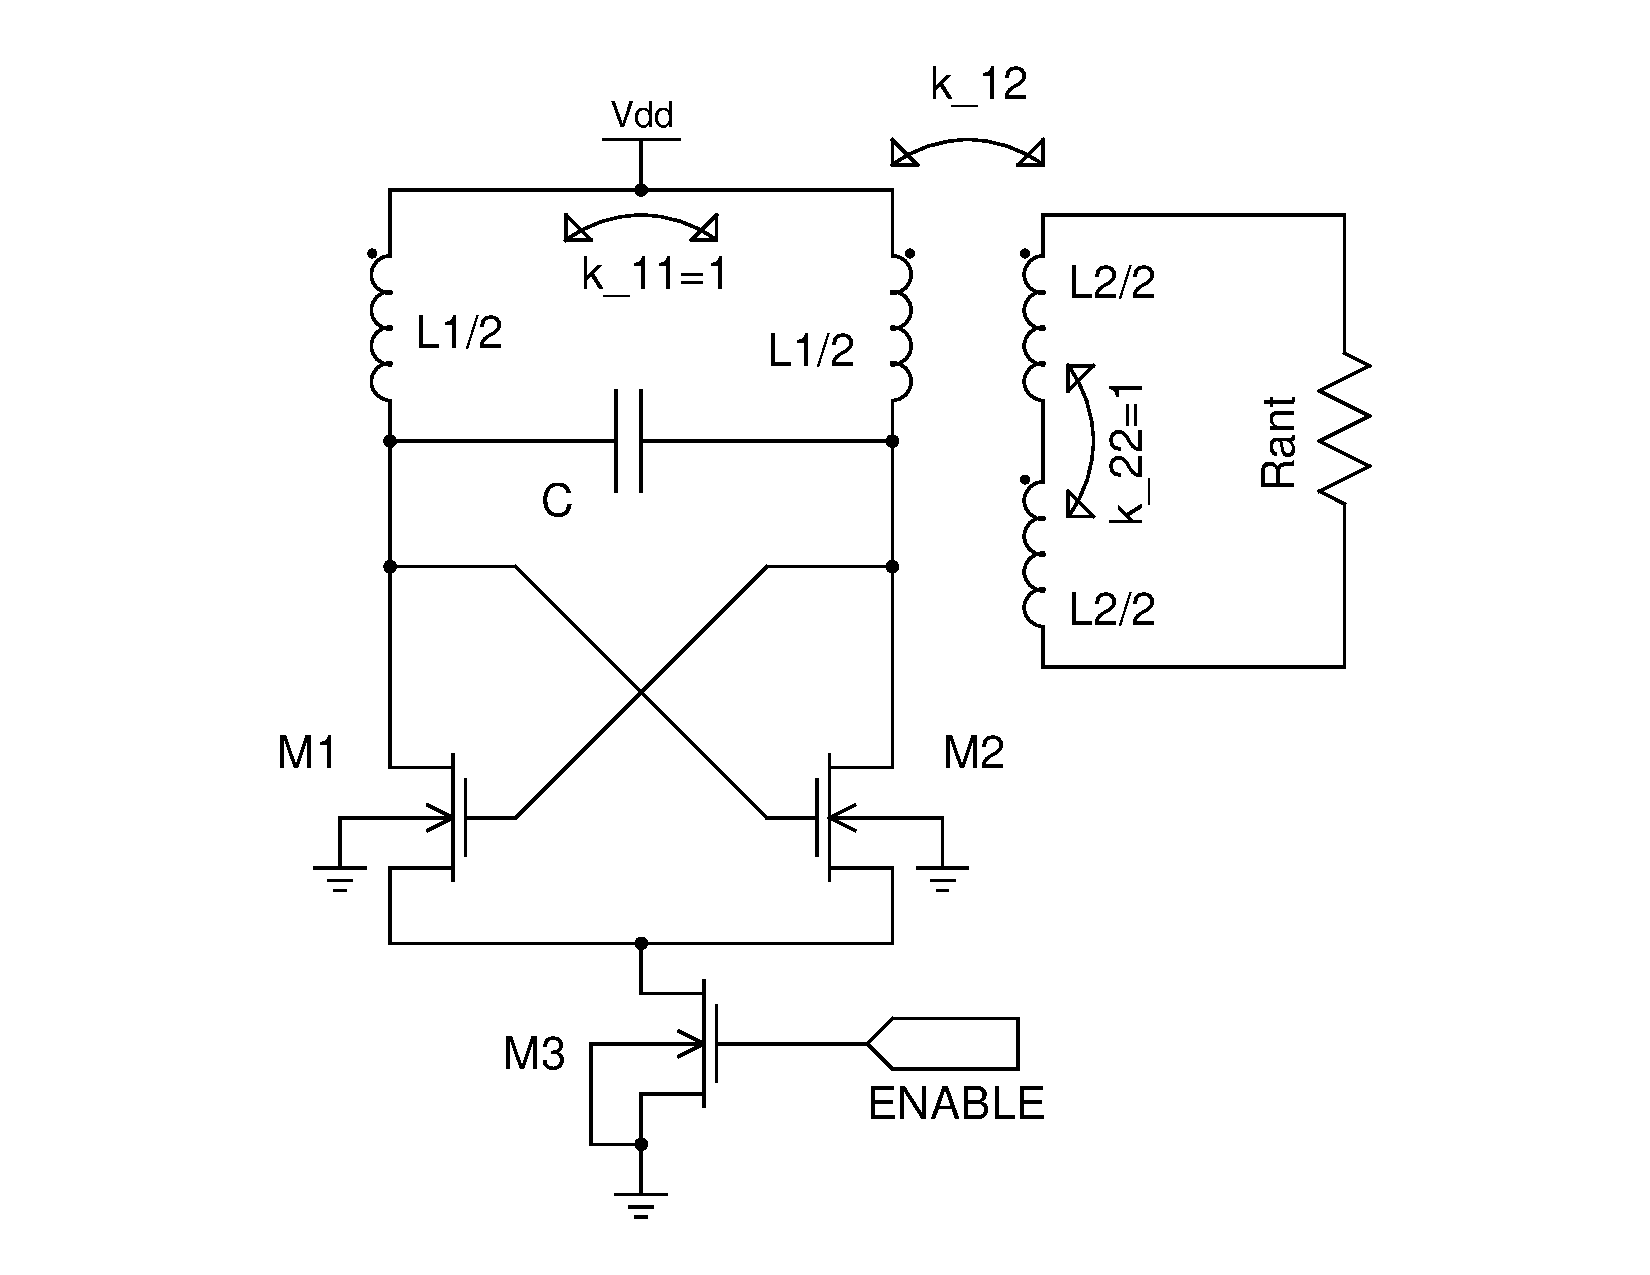
\includegraphics[width=0.67\textwidth]{images/tipo1.pdf}
\caption{Schema elettrico dell'oscillatore di Tipo 1. Si noti l' NMOS M3, la
      cui funzione è quella di connettere o disconnettere il circuito
	dall'alimentazione.}
\end{figure}
\begin{figure}[h]
\centering
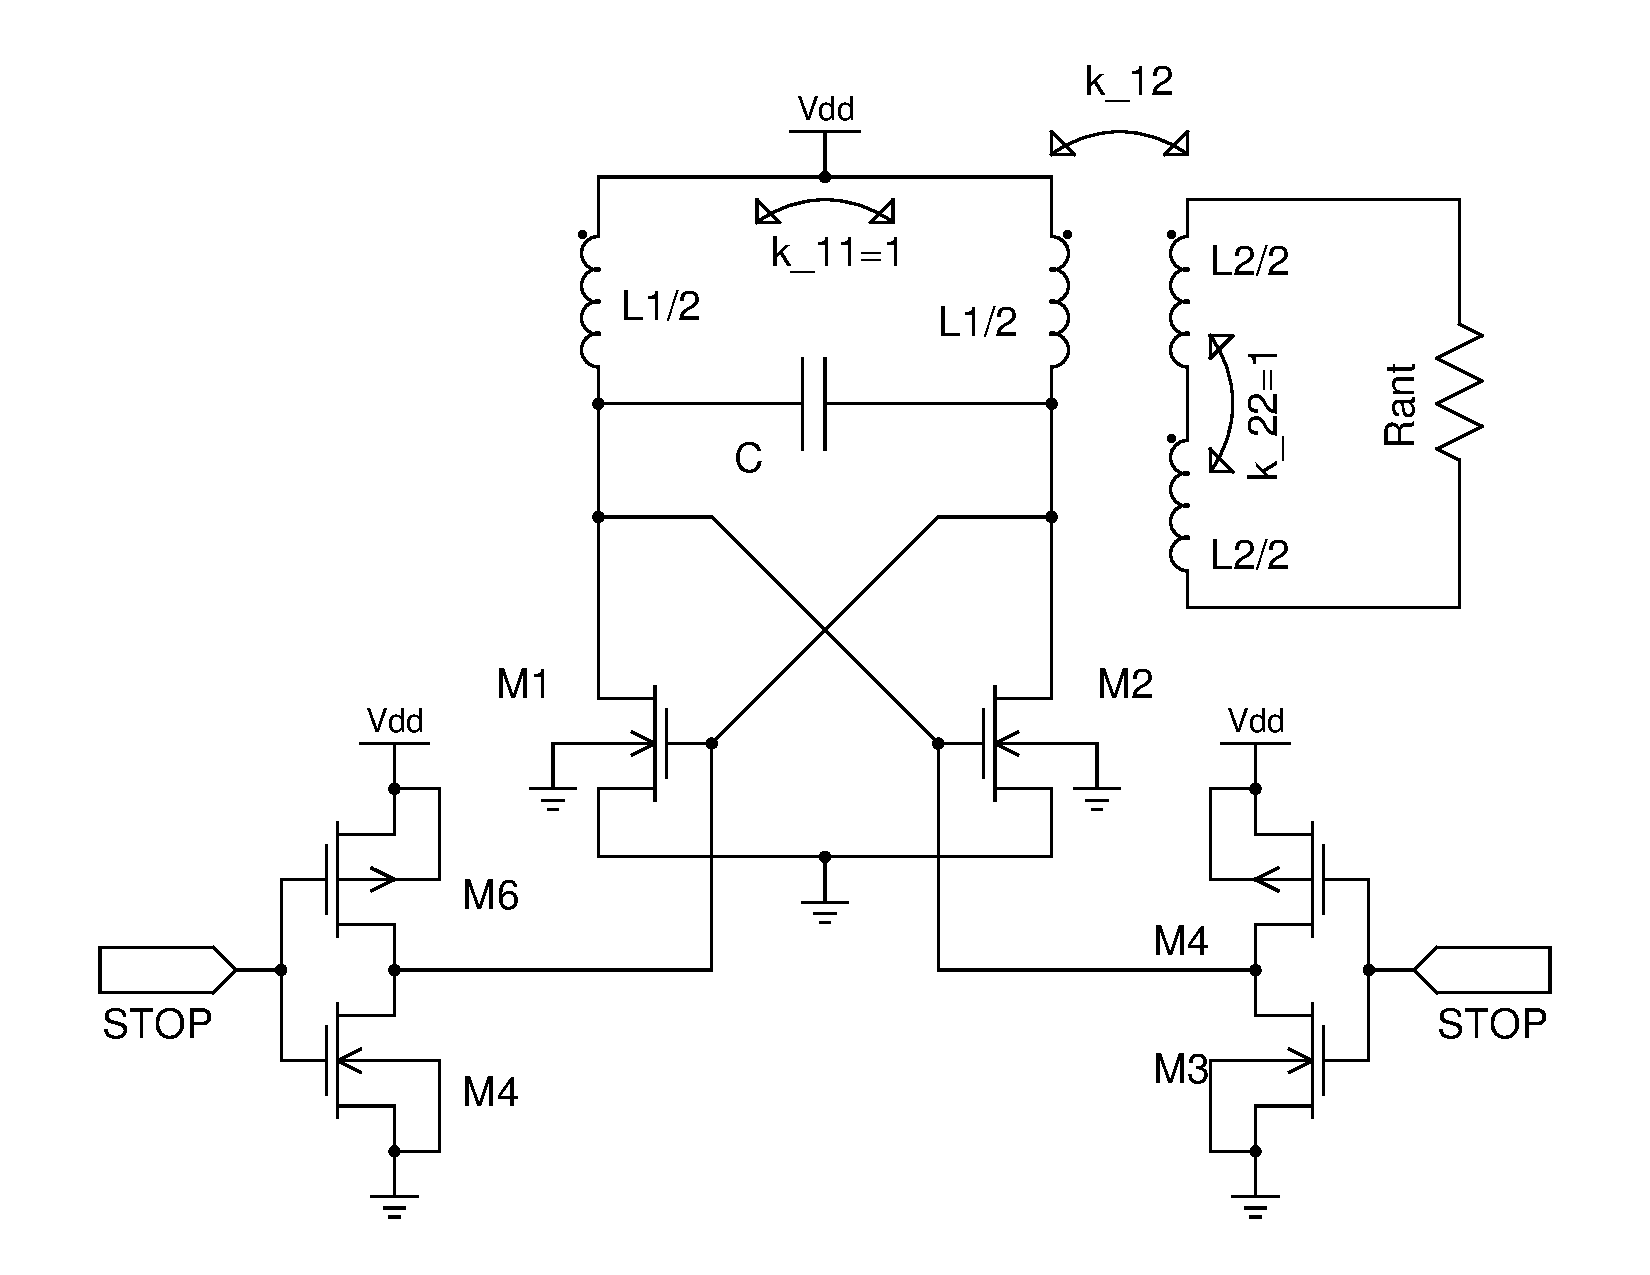
\includegraphics[width=0.75\textwidth]{images/tipo2.pdf}
\caption{Schema elettrico dell'oscillatore di Tipo 2. Gli invertitori CMOS
      connessi ai gate di M1 e M2 attivano o cortocircuitano a massa le
      oscillazioni.}
\end{figure}
\clearpage % leave space for the pictures

\noindent Quando \texttt{STOP} è alto sono attivi gli NMOS degli invertitori
che portano i \emph{gate} di M1 e M2 a massa, impedendo all'oscillatore di 
funzionare. Quando \texttt{STOP} è basso invece sono i PMOS ad essere attivi. I 
\emph{gate} di M1 e M2 sono ora connessi a Vdd tramite una resistenza di 
dimensioni dell'ordine della decina di Kiloohm per cui l'oscillatore viene 
attivato.

%%% TRASFORMATORE
\section{Il trasformatore}
Date le topologie di oscillatore presentate nella sezione precedente, il
trasformatore è l'elemento che più incide sull'efficienza della trasmissione.
Esso svolge infatti il ruolo fondamentale di trasformare, senza l'impiego di
ulteriori componenti attivi, la tensione differenziale presente al primario in
quella adatta a pilotare l'antenna\cite{Neviani14}.

Nei circuiti integrati induttanze e trasformatori sono realizzati come
spirali metalliche nello strato di \emph{metal} più superficiale (che è anche
lo strato più spesso).\\
A causa di questa loro struttura fisica si hanno dei componenti parassiti tra i
quali si annoverano\cite[pp. 431-455]{RazaviRF}:
\begin{description}
\item[capacità] tra le spire e il substrato, tra le spire e gli strati di
	\emph{metal} adiacenti e tra le spire stesse;
\item [resistori] dovuti alla resistenza serie del metallo che compone
	l'induttanza, all'effetto pelle e all'accoppiamento capacitivo con il
	substrato;
\item [induttori] dovuti all'accoppiamento magnetico con il substrato e con le 
	piste adiacenti.
\end{description}
Tutti questi parametri concorrono a degradare il fattore di qualità
dell'induttore.

Per effettuare le simulazioni è stato necessario produrre un modello per il
trasformatore che tenesse adeguatamente conto degli effetti sopracitati.\\
Si è valutato di restringere il campo ai soli elementi resistivi al fine di
ottenere dei dati semplificati utilizzabili per il confronto delle due
tipologie di oscillatore. L'inclusione degli altri elementi parassiti può
rappresentare uno stimolo per ulteriori studi e per affinare l'efficienza una
volta determinata la soluzione circuitale migliore.
\begin{figure}[h]
\centering
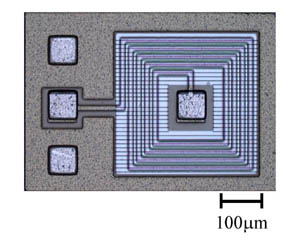
\includegraphics[height=0.2\textheight]{images/ic_inductor.JPG}
\caption{Microfotografia di un induttore in un circuito integrato
	\hspace{\textwidth} % force newline
	\footnotesize{Fonte: \url{http://people.seas.harvard.edu/~jones/es154
	/lectures/lecture_0}}}
\end{figure}

Il modello ottenuto per il trasformatore è presentato in Figura 2.4.
Tutti gli effetti indesiderati sono riassunti da una resistenza in serie al
primario divisa a metà tra i due rami. Tale resistenza è calcolata di volta in
volta, a partire dal valore di induttanza al primario, in modo da mantenere il
fattore di qualità Q a 25 per una frequenza di 8GHz.\\
La formula che lega il fattore di qualità al valore di $L_1$ è:
$ Q = 2\pi f_{osc} \frac{L_1}{R_p} $,\\
dove $R_p$ è la resistenza parassita al primario e $ f_{osc}=8GHz $.
\begin{figure}[h]
\centering
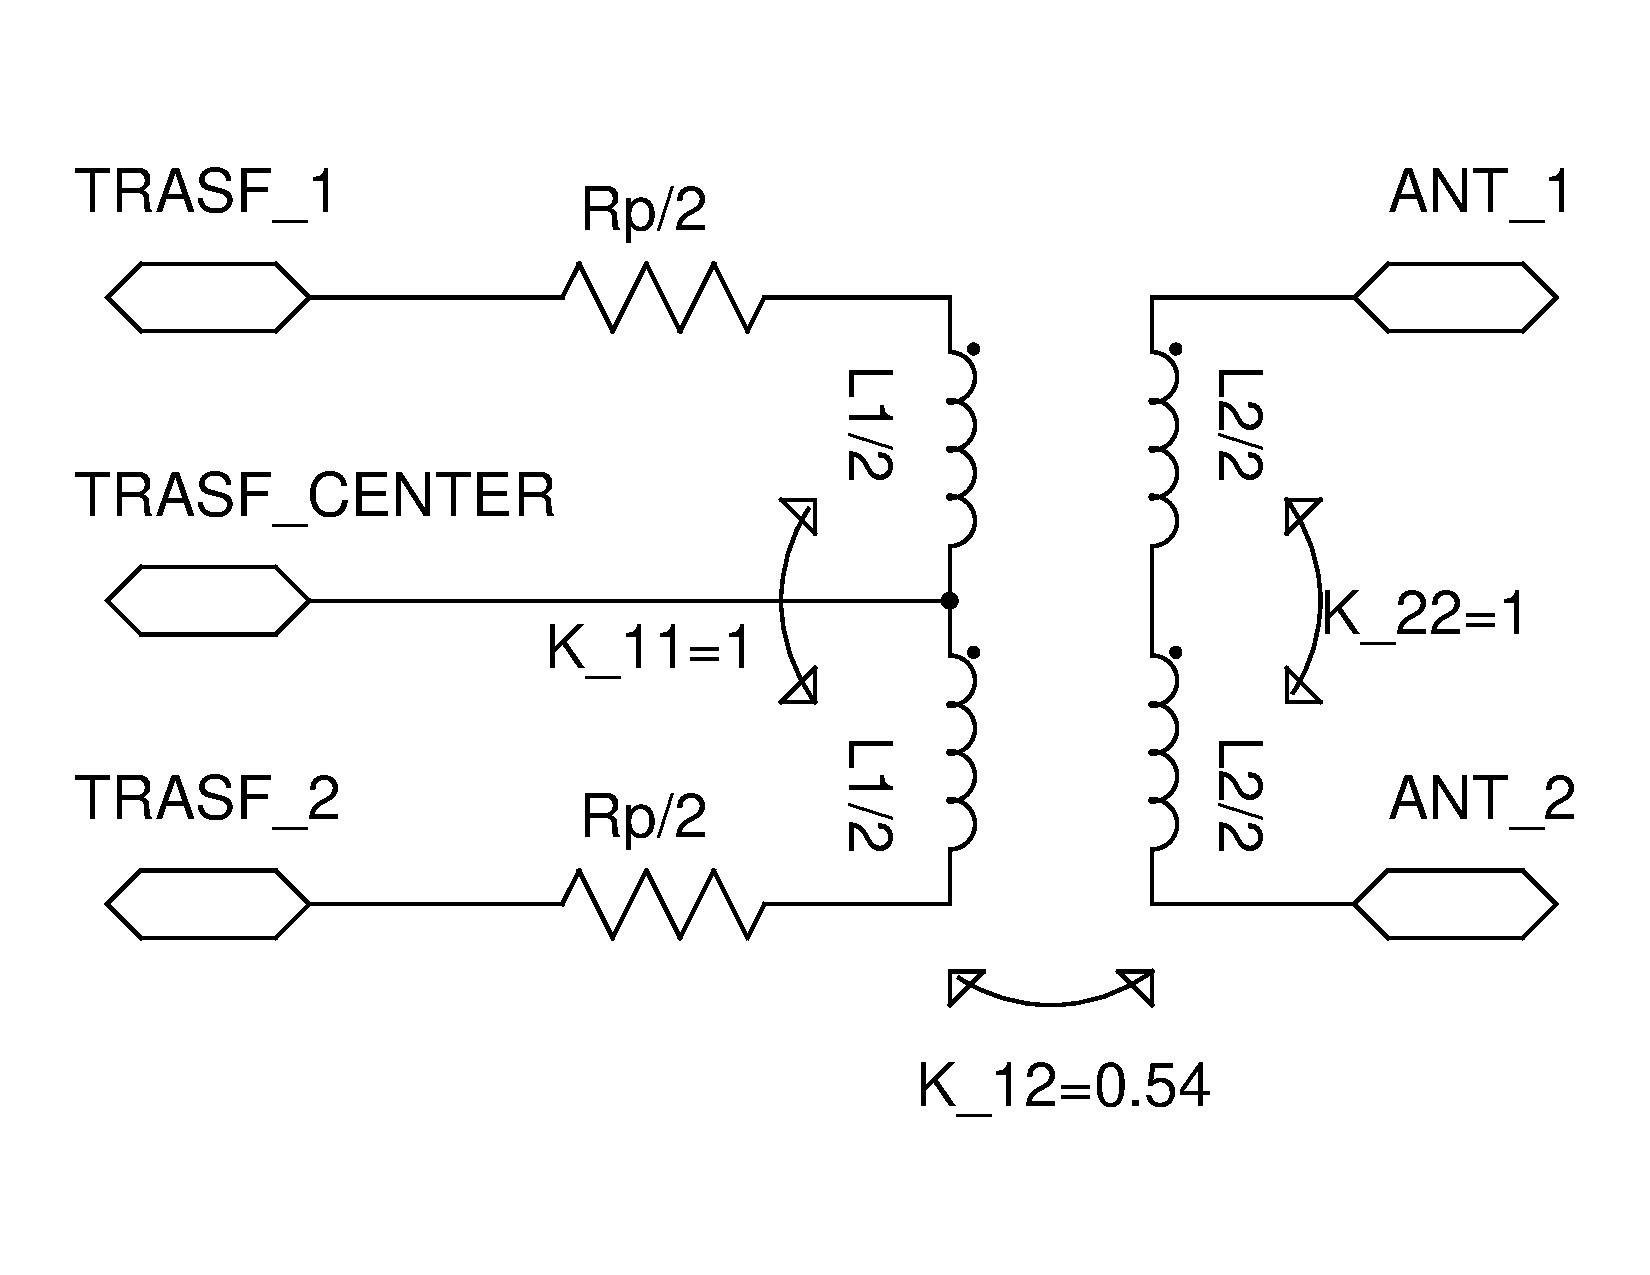
\includegraphics[height=0.34\textheight]{images/trasf_model.pdf}
\caption{Modello di trasformatore usato nelle simulazioni}
\end{figure}
\clearpage % pictures please

%%% MODELLO TEORICO
\section{Il modello teorico}
Per il lavoro di simulazione al calcolatore si è deciso di ricorrere 
all'analisi preliminare di un modello teorico che permettesse di valutare
qualitativamente i parametri che più influenzano l'efficienza energetica.\\
Il modello è stato utilizzato inoltre per confermare e supportare i risultati
emersi dalle simulazioni.

Si è partiti dall'oscillatore di Tipo 1 (Figura 2.1) e si sono formulate le
seguenti ipotesi:
\begin{enumerate}
\item l'oscillatore è attivo e si è esaurito l'effetto del transitorio
	iniziale;
\item il circuito funziona in regime limitato in tensione, ovvero l'ampiezza
	delle oscillazioni dipende solo dalla tensione di alimentazione;
\item la caduta di tensione sui componenti attivi del circuito è trascurabile;
\item il valore complessivo della capacità è tale da entrare in risonanza con
	l'induttanza totale del circuito.
\end{enumerate}
L'ipotesi 1. è dettata dal fatto che nel presente elaborato si valuta 
l'efficienza a regime dell'oscillatore, trascurando la potenza dissipata per
produrre gli impulsi.\\
L'ipotesi 2. è ragionevole se gli NMOS sono adeguatamente dimensionati e dunque
al primario si ha un'oscillazione differenziale di ampiezza $2V_{DD}$.\\
L'ipotesi 3. è utile per restringere l'analisi al solo trasformatore e sarà
rilassata in seguito.\\
L'ipotesi 4. è suffragata dalla natura stessa del funzionamento 
dell'oscillatore che lavora alla frequenza di risonanza tra induttanza e
capacità presenti nel circuito.
\begin{figure}[h!]
\centering
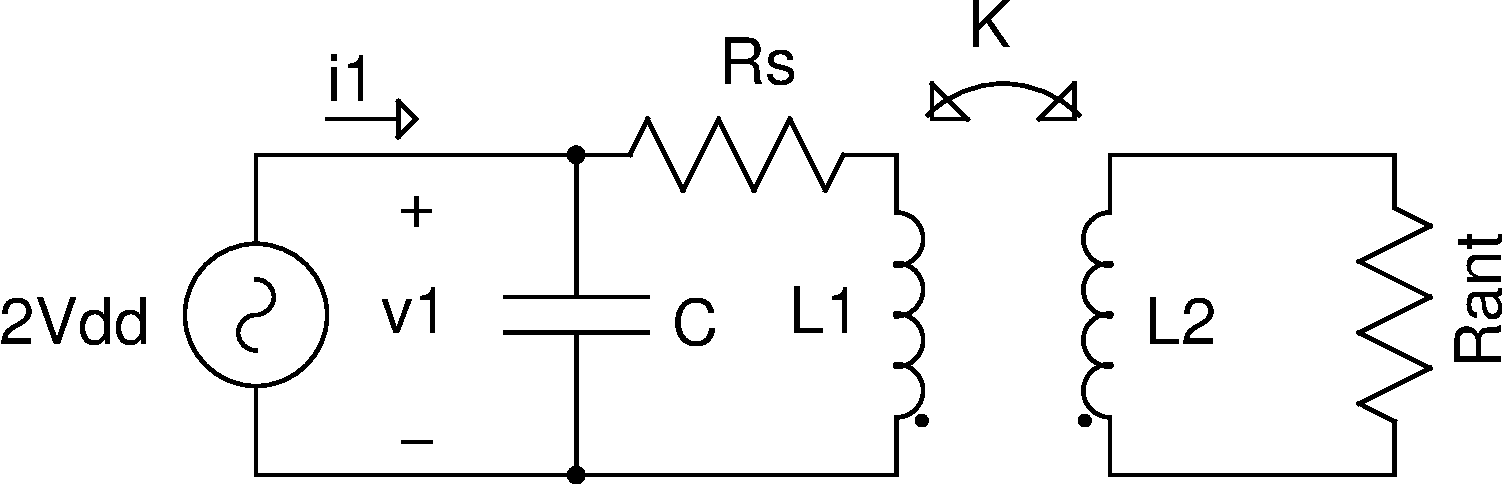
\includegraphics[height=0.12\textheight]{images/cir_model.pdf}
\caption{Modello teorico dell'oscillatore}
\end{figure}

Tali ipotesi permettono di approssimare il circuito con un generatore
ideale di tensione sinusoidale di ampiezza $2V_{DD}$, connesso alla serie tra
una resistenza e il primario di un trasformatore. Il secondario è connesso
direttamente alla resistenza di antenna (Figura 2.5).

Al circuito così ottenuto si possono applicare le relazioni che permettono di
passare dal doppio bipolo induttivo al trasformatore ideale con induttanza in
eccedenza\cite[pp. 322-323]{GuarnieriET}. Sfruttando poi le proprietà del
trasformatore ideale si ottiene la Figura 2.6,
\begin{figure}[H]
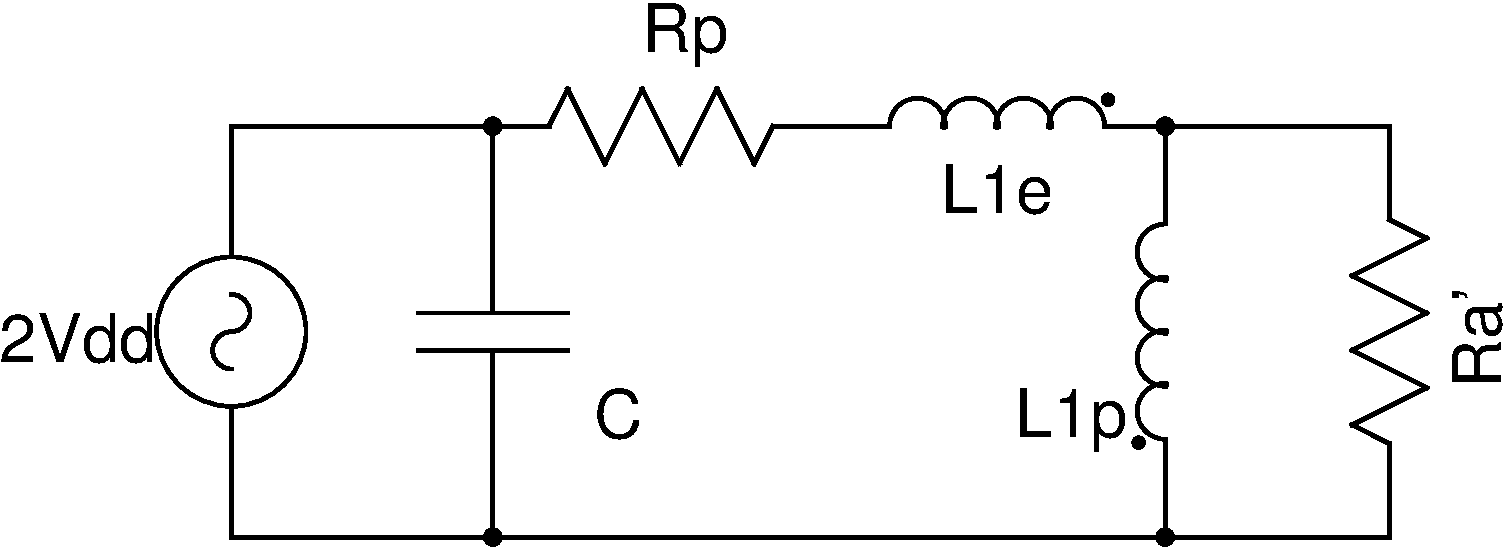
\includegraphics[width=0.55\textwidth]{images/cir_model1.pdf}
\centering
\caption{}
\end{figure}
\noindent in cui le espressioni dei valori dei componenti sono:
\begin{description}
\item $ R_p = 2 \pi f_{osc} \frac{L_1}{Q} $
\item $ L_{1p} = K^2 L_1 $
\item $ L_{1e} = \left( 1 - K^2 \right) L_1 $
\item $ n' = \sqrt{\frac{L_{1p}}{L_2}} = K \sqrt{\frac{L_1}{L_2}} = Kn $
\item $ R_a' = {\left( nk \right)}^2 R_a $
\end{description}

Si applicano infine le trasformazioni serie-parallelo\cite[pp. 63-64]{RazaviRF}
per la serie di $R_p $ e $L_{1e}$. Sapendo inoltre che per l'ipotesi 4. 
la capacità e le induttanze sono in risonanza, il circuito che si determina è
rappresentato in figura 2.7. 
\begin{figure}[H]
\centering
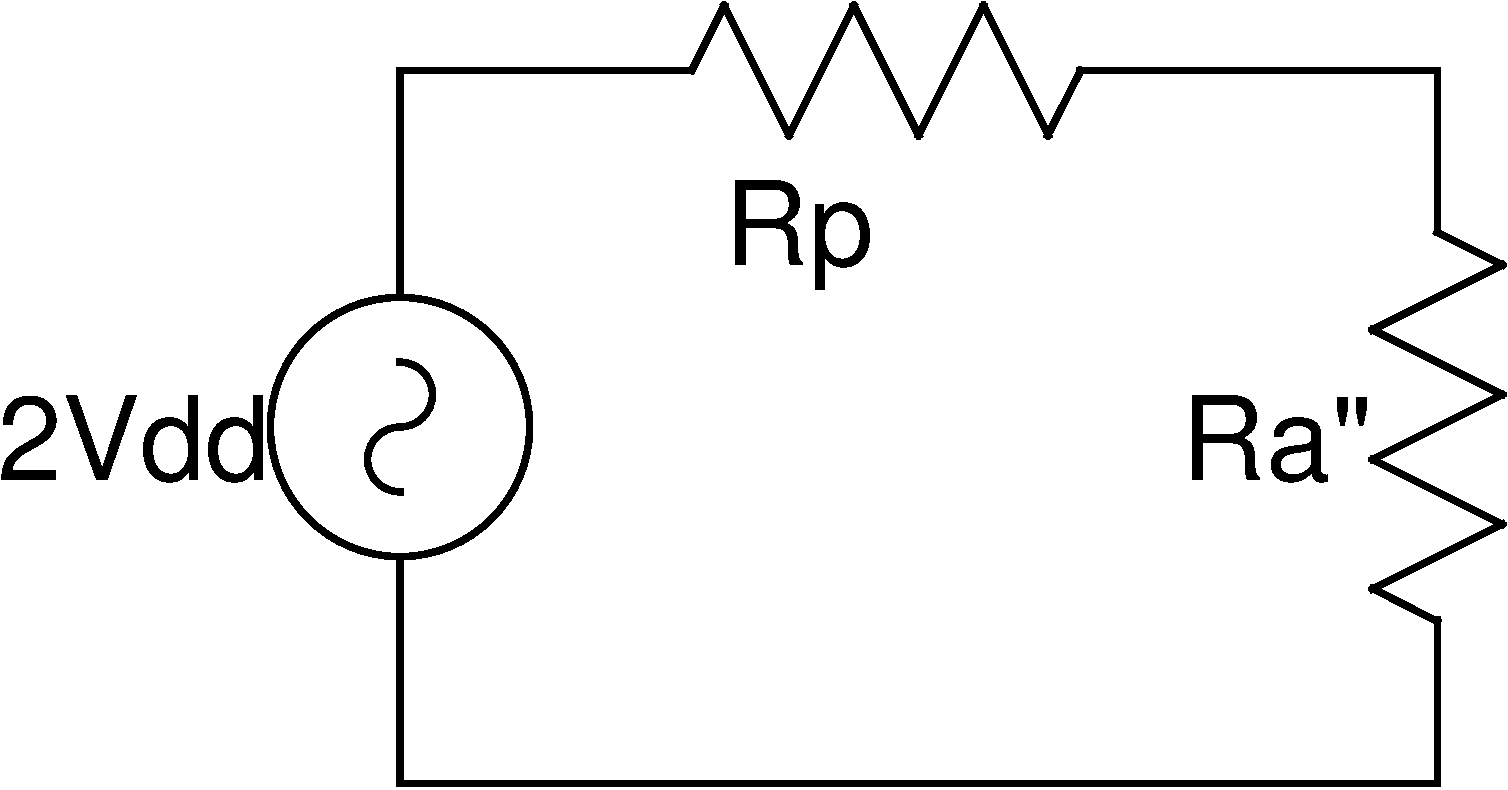
\includegraphics[width=0.35\textwidth]{images/cir_model2.pdf}
\caption{}
\end{figure}

\noindent Nella figura è rappresentato un partitore di corrente.\\
Il  valore di $ R_p' $ è: $ R_p' = R_p \left(1 + Q^2 \right) $.\\
L'efficienza è dunque:
{\large$ \eta_t = \frac{P_{ant}}{P_{tot}} = \frac{R_p (1 + Q^2)}{n'R_a + 
(1 + Q^2)R_p} $}
\\Sostituendo a $R_p$ ed $n'$ le rispettive espressioni si ottiene:
$$ \eta_t = \frac{2\pi f_{osc} L_2 (\frac{1}{Q} + Q)}
{2\pi f_{osc}L_2(\frac{1}{Q} + Q) + K^2R_a } $$

Dalla precedente formula si evince come, in prima approssimazione, l'efficienza
teorica sia solo funzione del fattore di qualità Q, del fattore di 
accoppiamento K e dell'induttanza al secondario $L_2$.\\
L'unico di questi parametri che sia accessibile in fase di progetto è il
valore di $L_2$ in quanto  gli altri sono determinati dal \emph{layout} del
trasformatore.\\
L'efficienza teorica tende ad uno per $L_2$ che tende all'infinito. Il valore
di $L_2$ deve dunque essere il più elevato possibile.

Una volta isolato il contributo del trasformatore è possibile dedicarsi 
all'effetto introdotto dai componenti attivi nel circuito.\\
L'efficienza complessiva a regime è infatti il prodotto dell'efficienza del
trasformatore ($\eta_t$) per l'efficienza dei componenti attivi ($\eta_a$):
$ \eta = \eta_t \eta_a $.

Con riferimento alla Figura 2.1 si ha che M3 è sempre attivo per l'ipotesi 1;
M1 ed M2 invece conducono esattamente per metà del ciclo di oscillazione.\\
Approssimando i \emph{transistor} con degli interruttori, dalla loro attività
si ottiene un' onda quadra.\\
Ricorrendo al termine del primo ordine dello sviluppo in serie di Fourier, 
l'efficienza relativa ai componenti attivi può essere espressa dalla formula:
\cite{Neviani14}$$ \eta_a=\frac{\frac{2}{\pi}\left(V_{DD}-V_{DS,1}-V_{DS,3}
\right)}{V_{DD}}$$

Supponendo di aver dimensionato gli NMOS in modo tale che la caduta di tensione
tra \emph{drain} e \emph{source} sia trascurabile rispetto all'ampiezza delle
oscillazioni ai loro capi\footnote{Nel capitolo seguente le simulazioni
effettuate confermeranno la veridicità di questo assunto} si ha che: {\large 
$\eta_a \approx \frac{2}{\pi} \approx 0,63$}. Tale valore rappresenta anche la
massima efficienza teoricamente raggiungibile.
\begin{figure}[h]
\centering
\includegraphics[height=0.4\textheight]{effteor.pdf}
\caption{Efficienza per il modello teorico al variare di $L_2$ ($f_{osc} = 8GHz 
$ e $K=0.54 $).}
\end{figure}

%%% PARAMETRI DI INTERESSE
\section{Parametri di interesse}
Nella presente sezione si analizzano e discutono i componenti il cui valore ha
un' influenza sull'efficienza della trasmissione dal punto di vista qualitativo.
\\Al fine di snellire la trattazione si è ritenuto necessario dividere 
l'analisi nei tre ambiti: trasformatore e capacità, oscillatore di Tipo 1 e
oscillatore di Tipo 2.

\subsection{Trasformatore e capacità}
Con riferimento alle figure 2.1, 2.4 e 2.7 si individuano:
\begin{enumerate}
\item[L1], ovvero l'induttanza al primario. Da essa dipende direttamente il
	valore della resistenza parassita vista ai terminali \texttt{TRASF\_1} e
	\texttt{TRASF\_2}.\\
	Come precedentemente discusso, la resistenza parassita di $L_1$ può essere
	convertita, tramite le trasformazioni serie-parallelo, in una resistenza
	in parallelo all'antenna.\\
	Dal momento che la corrente erogata dal circuito nel trasformatore si
	divide tra la resistenza parassita e l'antenna, è necessario che il
	valore di $R_p'$ sia molto maggiore rispetto a $R_a'$.\\
	Dall'analisi effettuata nella sezione precedente si desidera $L_2$ grande,
	il che porta $n'$ ad essere piccolo e dunque anche $R_a' = n'R_a$ avrà un
	valore dell'ordine di grandezza dell'ohm.\\
	Essendo $R_p' = 2\pi f_{osc} L_1 \left(\frac{1}{Q} + Q \right)$, $L1$ deve
	essere sufficientemente grande da rendere $R_p' \gg R_a'$.\\
	Un valore troppo grande di $L1$ tuttavia aumenta la corrente che scorre
	nel primario e dunque nei MOSFET del circuito. Se questi ultimi non sono
	in grado di sopportare tali correnti la caduta di potenziale su di essi
	si fa rilevante causando una drastica perdita di efficienza e il
	passaggio da regime limitato in tensione a regime limitato in corrente.

\item[L2], ovvero l'induttanza al secondario. Da essa dipende il rapporto di
	trasformazione e l'efficienza complessiva del trasformatore.\\
	Per la sua induttanza il modello teorico richiede un valore elevato, al
	limite infinito.\\
	Nel processo CMOS il fattore di qualità di un induttore degrada
	rapidamente all'aumentare del numero di spire e della dimensione
	dell'induttore stesso, sia a causa dell'elevata resistività delle piste
	sia a causa dei contributi capacitivi\cite{RazaviRF}.\\
	Un basso fattore di qualità al secondario aumenta l'energia dissipata
	nell'induttanza, a scapito di quella erogata all'antenna.\\
	All'aumentare di $L_2$ diminuisce il rapporto di trasformazione e con
	esso la resistenza che deve essere pilotata dagli NMOS.\@ Analogamente a
	quanto affermato per $L_1$ una corrente troppo elevata che scorre nei
	componenti attivi va a detrimento dell'efficienza.

\item[C], ovvero la capacità del \emph{tank}. Da essa e dall'induttanza
	complessiva dipendono la frequenza di oscillazione e il
	\emph{tuning-range} (intervallo di frequenze che può essere coperto
	dall'oscillatore al variare di C, utile per recuperare variazioni nei
	valori dei componenti causati dagli errori del processo).\\
	La formula $ f_{osc}=\frac{1}{2\pi\sqrt{L_{tot}C_{tot}}}$ determina la
	frequenza di oscillazione (si veda capitolo 1).
	\\Il \emph{tuning-range} è definito come: $ R = f_{osc}^{(max)} -
	f_{osc}^{(min)} $.\\
	Valori elevati di $L_{tot}$ riducono l'influenza di C sulla massima e
	minima frequenza raggiungibile. \`E dunque necessario scegliere il valore
	nominale di C in modo da garantire l'oscillazione a $8GHz$, avendo
	fissato $L1$ ed $L2$ ad un valore tale da ottenere il \emph{tuning-range}
	desiderato.
\end{enumerate}

\subsection{Oscillatore di Tipo 1}
Con riferimento alla Figura 2.1, una volta determinati i parametri ottimali per
il trasformatore, è necessario assicurarsi che la caduta di tensione sugli NMOS
sia trascurabile. Per fare ciò si aumenta il fattore di forma $Z = \frac{W}{L}$
di M1 ed M2.\\
Un fattore di forma troppo elevato, oltre ad incidere sull'area occupata dal 
circuito, rende elevata la capacità parassita introdotta dagli NMOS degradando
il \emph{tuning-range} e costringendo ad impiegare induttanze più piccole che,
come si è visto riducono l'efficienza della trasmissione.

Fondamentale è la dimensione di M3, scelta in modo che la caduta di tensione
tra \emph{drain}e \emph{source} sia trascurabile e, ai piccoli segnali, il nodo
in cui si incontrano i \emph{source} di M1 2 M2 si possa considerare a massa.

Ricorrendo ad un M3 con fattore di forma elevato si ha un aumento dell'energia
dissipata dalla circuiteria di controllo per accendere e spegnere il circuito.
Aumenta inoltre il tempo di ritardo tra l'arrivo del segnale di controllo e 
l'accensione o lo spegnimento dell'oscillatore.

\subsection{Oscillatore di Tipo 2}
Con riferimento alla Figura 2.2, per M1 ed M2 valgono le medesime
considerazioni rispetto al Tipo 1.
Due invertitori sono connessi ai \emph{gate} di tali MOSFET.

Affinché l'oscillatore possa essere spento M3 ed M4 devono avere dimensioni 
comparabili o maggiori di M1 ed M2, altrimenti il loro contributo non è 
sufficiente a fermare le oscillazioni.\\
I PMOS invece devono essere fortemente resistivi in modo che la loro resistenza
non imponga un carico eccessivo su M1 ed M2.

Il dimensionamento troppo elevato dei transistor che compongono l'invertitore
aumenta la capacità vista dalla circuiteria di controllo e rallenta il tempo di 
risposta al segnale di attivazione e spegnimento.\\
\`E dunque auspicabile per i PMOS una dimensione minima e per gli NMOS 
dell'invertitore una dimensione di poco più grande rispetto a quella dei
\emph{transistor} dell'oscillatore.
%%%%%%%%%%%%%%%%%%%%%%%%%%%%%
% Risultati numerici
%%%%%%%%%%%%%%%%%%%%%%%%%%%%%
\chapter{Risultati numerici}
Sono state effettuate tre tipologie di simulazioni distinte:
\begin{itemize}
\item La prima parte dall'oscillatore di Tipo 1 con gli stessi parametri
	circuitali in \cite{Neviani14}, adattati al modello di trasformatore 
	utilizzato. Questa rappresenta il punto di partenza e porge un'efficienza
	in trasmissione pari al 10\%. A partire da questo valore si è fatto
	variare il rapporto di trasformazione e il valore delle induttanze al
	primario e secondario del trasformatore. L'efficienza massima raggiunta è
	pari al 29,4\%.

\item La seconda impiega gli stessi valori dei componenti del trasformatore,
	questa vola applicati all'oscillatore di Tipo 2. In questa simulazione ci
	si è concentrato sul dimensionamento degli invertitori e l'efficienza
	massima raggiunta è pari al 28,1\%.

\item L'ultima mira a confrontare qualitativamente il comportamento in caso di
	funzionamento impulsato, confrontando i tempi di accensione e spegnimento
	dei due oscillatori.
\end{itemize}
Segue una disamina dettagliata del lavoro svolto.

%% TIPO 1
\section{Tipo 1}
In Figura 3.1 si può osservare l'efficienza totale del circuito simulato al
calcolatore per diversi valori dell'induttanza $L_1$ e $L_2$. Sono inoltre
presenti delle rette che rappresentano diversi valori per il rapporto di
trasformazione.
\begin{figure}[h!]
\centering
\includegraphics[width=\textwidth]{efficienza.pdf}
\caption{}
\end{figure}

Si è notato un generale aumento di efficienza per $L_2$ crescente.\\
Come si evince dal modello teorico ciò è dovuto alla maggiore corrente che 
scorre nella resistenza di antenna piuttosto che in quella parassita.\\
Si ha inoltre un aumento dell'efficienza al diminuire di $L_1$, finché non è
raggiunto il valore di $70pH$, oltre al quale l'efficienza inizia a diminuire.
\\Questo comportamento è in accordo con il modello teorico, il quale prevede
che l'efficienza aumenti per $L_1$ grande.  Tuttavia all'aumentare 
dell'induttanza al primario aumenta la corrente che circola nei MOSFET e con
essa aumenta quella assorbita dal circuito.\\
Questo fenomeno, oltre a degradare l'efficienza impone un carico eccessivo sui
transistor che non sono più in grado di pilotare adeguatamente il trasformatore.
Le simulazioni hanno evidenziato come valori di $L_1$ pari o superiori a $200pH$
sono troppo elevati e producono, oltre che una scarsa efficienza, un'onda
sinusoidale piuttosto distorta all'antenna.\\
Si ha perciò che il valore ottimale per $L_1$ è pari a $70pH$.
\begin{figure}[h!]
\centering
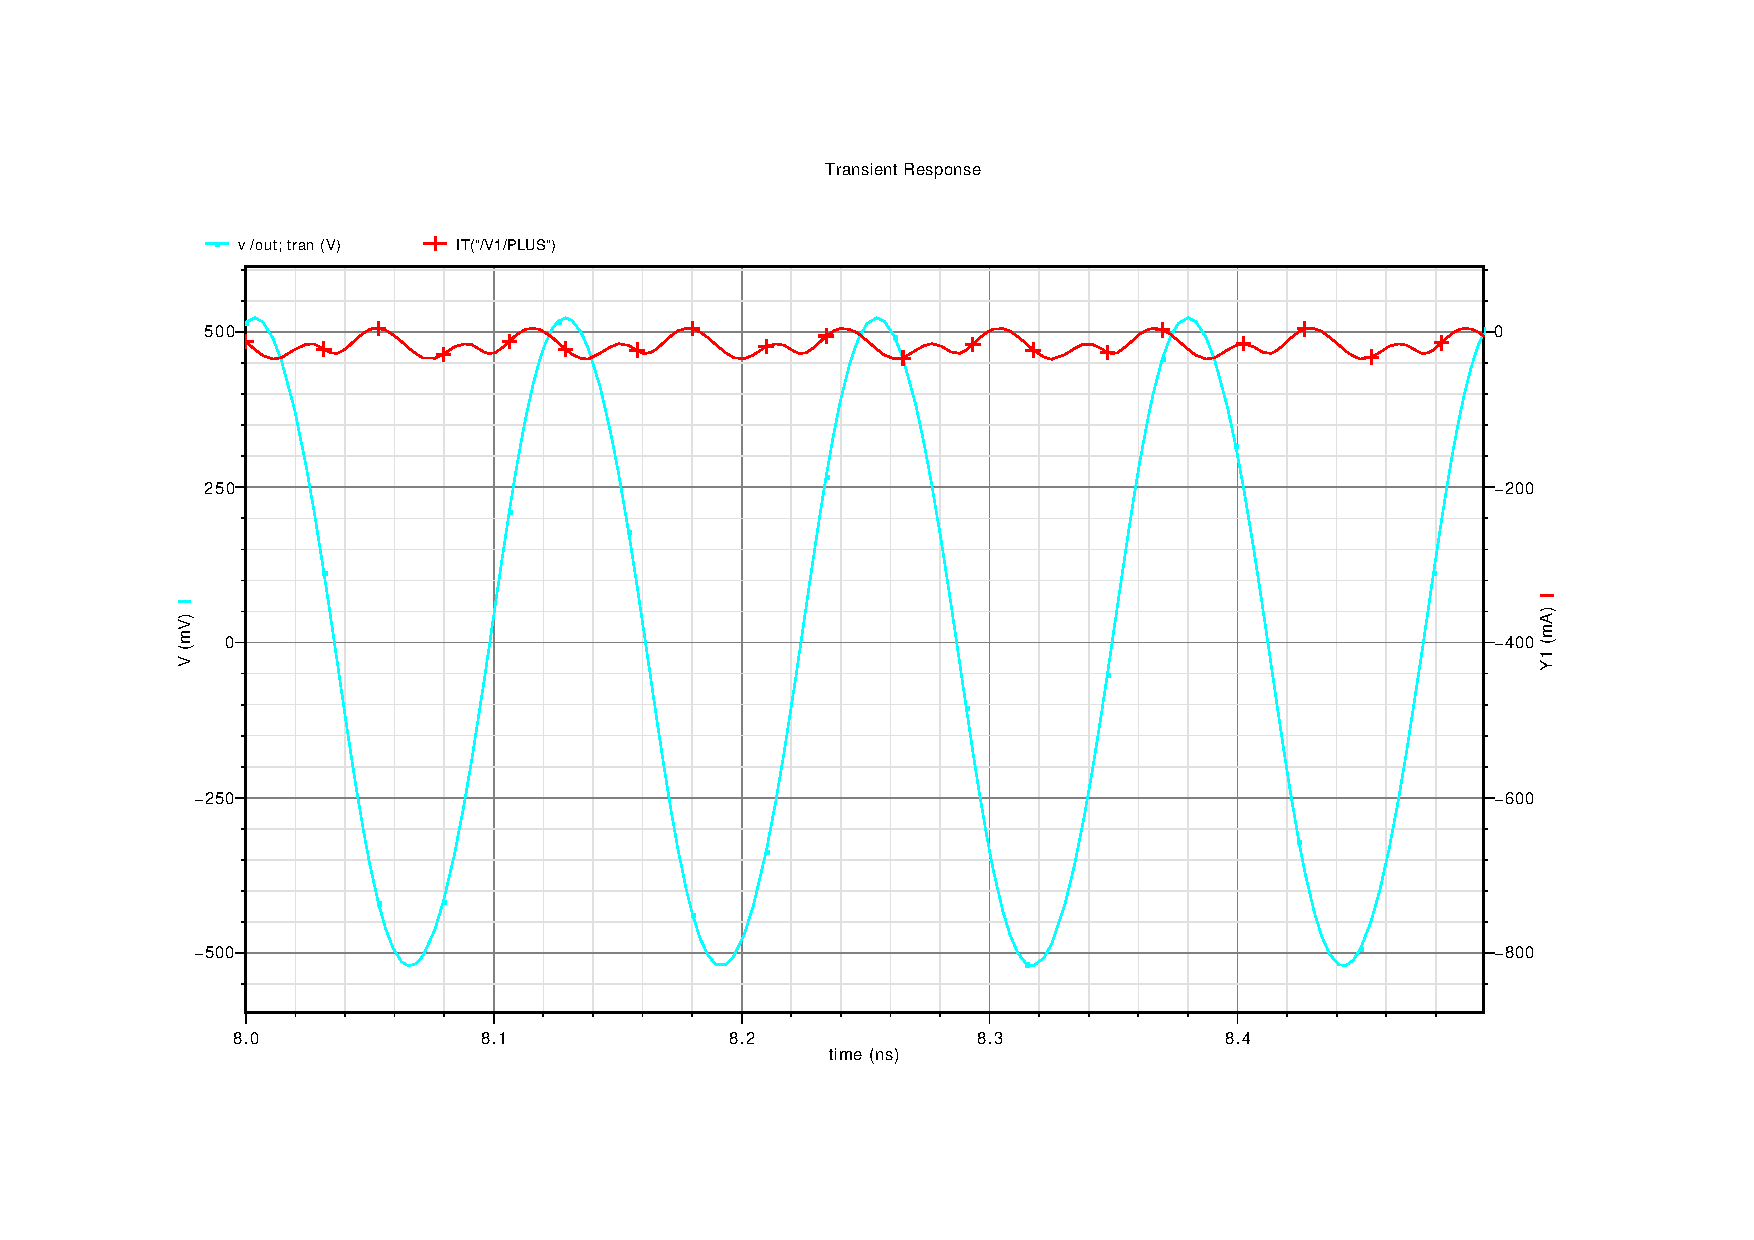
\includegraphics[width=\textwidth]{images/Vant-It.pdf}
\caption{Tensione all'antenna e corrente assorbita per l'oscillatore di Tipo 1
      con dimensioni ottimali per il trasformatore.}
\end{figure}
\clearpage

Il valore iniziale per il rapporto di trasformazione era $n_{iniziale}=1,155$
il quale porge un'efficienza pari al 10\% (valore indicato dalla freccia in
figura).\\
Portando il rapporto di trasformazione a $n_{ottimo}=0,42$ e impostando
$L_1=70pH$ e $L_2=400pH$ si è raggiunta la migliore figura di efficienza, pari
al $29,4\%$.\\

%% TIPO 2
\section{Tipo 2}
%%%%%%%%%%%%%%%%%%%%%%%%%%%%%
% Conclusione e sviluppi futuri
%%%%%%%%%%%%%%%%%%%%%%%%%%%%%
\cleardoublepage{}
\chapter{Conclusione}

\section{Sviluppi futuri}

%%%%%%%%%%%%%%%%%%%%%%%%%%%%%
% Bibliografia
%%%%%%%%%%%%%%%%%%%%%%%%%%%%%
\bibliographystyle{plain}
\bibliography{tex/biblio}
\end{document}
